
\documentclass{article}
\usepackage{iclr2025_conference,times}

\input{math_commands.tex}

\usepackage{hyperref}
\usepackage{url}
\usepackage{amsmath}
\usepackage{graphicx}
\usepackage{booktabs}
\usepackage{microtype}

\title{GeoAgent: Iterative Reasoning and \\ Tool Integration for Remote Sensing \\ Vision-Language Models}

\author{%
  Alperen Enes Bayar \\
  Student ID: N24142767 \\[0.5ex]
  \textbf{Course:} Computer Vision (CMP719) \\
  \textbf{Instructor:} Prof.\ Naz\-l{\i} \. Ikizler-Cinbi\c{s}
}

\newcommand{\fix}{\marginpar{FIX}}
\newcommand{\new}{\marginpar{NEW}}

\iclrfinalcopy

\begin{document}

\maketitle

\begin{abstract}
Large vision-language models (VLMs) applied to remote sensing imagery typically
operate in a single-pass inference regime: a question is posed, the model produces
a response, and no further deliberation occurs.  This design is ill-suited to
geospatial queries that require progressive spatial attention or multi-step
reasoning.  We present \textbf{GeoAgent}, an iterative reasoning layer built atop
GeoChat \citep{kuckreja2024geochat}, a grounded VLM pre-trained on diverse remote
sensing data.  GeoAgent replaces single-pass inference with a structured decision
loop: at each step the model outputs a JSON control object specifying whether to
invoke a spatial tool (e.g.\ region cropping), emit an intermediate observation,
or terminate with a final answer.  Across iterations a persistent
\texttt{GeoAgentMemory} structure accumulates observations and step traces; if the
planner does not self-terminate within a fixed budget, a final summarisation pass
synthesises the accumulated context into a concise response.  We evaluate GeoAgent
on Remote Sensing Visual Question Answering (RSVQA LR and HR) and on aerial scene
classification (UCMerced, AID).  GeoAgent improves average RSVQA accuracy from
90.70\% to 92.29\% with no additional fine-tuning, and yields comparable or
improved accuracy on AID (72.03\%\,$\to$\,73.00\%).  These results demonstrate
that agentic, tool-augmented reasoning can meaningfully augment a state-of-the-art
remote sensing VLM without modifying its weights.
\end{abstract}

% ---------------------------------------------------------------------------
\section{Introduction}
\label{sec:intro}
% ---------------------------------------------------------------------------

Remote sensing imagery---acquired by satellites, aircraft, and drones---is a
primary data source for land-cover classification, disaster response, urban
planning, and environmental monitoring.  Despite the richness of information these
images carry, accessing that information traditionally requires expert knowledge:
analysts must select and parameterise task-specific models and interpret outputs
manually.  A more accessible paradigm would allow users to pose queries in natural
language and receive accurate, grounded answers directly from the imagery.

Vision-language models (VLMs) offer a promising pathway toward this goal.  By
jointly representing visual and linguistic information, models such as
LLaVA~\citep{liu2023llava} and InstructBLIP~\citep{dai2023instructblip} enable
open-ended visual question answering (VQA) across general image domains.  Extending
this capability to remote sensing is non-trivial: aerial imagery differs
fundamentally from natural photographs in scale, resolution, object density, and
the spatial relational structure of queries (e.g., ``How many buildings are
adjacent to the river?'').  GeoChat~\citep{kuckreja2024geochat} addresses this gap
by training a grounded VLM on a large-scale, instruction-following dataset curated
specifically for remote sensing, enabling spatial referencing and region-aware
conversation.

Despite its strong empirical performance, GeoChat---like most VLMs---operates in a
\emph{single-pass} inference regime: the model is presented with an image and a
query, produces a response, and terminates.  This is adequate for queries whose
answer is directly visible in the scene at the presented resolution.  However, it
is ill-suited to questions that require the model to zoom into a sub-region,
integrate evidence across multiple spatial scales, or iteratively narrow attention
to a specific entity.  Such multi-step spatial reasoning is common in operational
remote sensing workflows yet absent from standard VLM inference pipelines.

In this paper we introduce \textbf{GeoAgent}, an agentic extension of GeoChat that
transforms single-pass inference into a structured, multi-step decision loop.
GeoAgent is inspired by the ReAct framework~\citep{yao2023react}, which interleaves
reasoning traces with executable actions.  At each iteration the GeoChat backbone
is prompted to emit a JSON control object specifying one of three actions:
\textit{tool call} (e.g., crop a sub-region, rotate to a canonical orientation,
enhance image contrast, or detect structural edges), \textit{direct answer}, or
\textit{stop}.  A lightweight memory structure persists observations and step traces
across iterations, and a final summarisation pass produces a concise answer from the
accumulated context when the planner does not self-terminate.  The tool interface is
modular: the default prototype ships with four spatial and enhancement tools, but
custom tools conforming to a simple protocol can be registered without modifying the
core loop.

\paragraph{Contributions.}
\begin{enumerate}
  \item \textbf{GeoAgent}: a modular, training-free agentic reasoning layer for
    remote sensing VLMs that enables iterative spatial reasoning via structured
    action planning and tool invocation.  The default tool set comprises four
    complementary operations: region cropping, image rotation, contrast
    enhancement, and edge detection.
  \item \textbf{GeoAgentMemory}: a persistent memory structure that accumulates
    per-step observations and decisions, enabling multi-step context integration
    and final-answer synthesis.
  \item Empirical evaluation on RSVQA~(LR \& HR) and aerial scene classification
    (UCMerced, AID), demonstrating consistent VQA gains with no additional
    training.
  \item \textbf{Confidence-gated routing and step-confidence aggregation}:
    an entropy-based gate that suppresses the agent loop for high-confidence
    queries, and a mean log-probability selection criterion that chooses the
    most confident intermediate answer across reasoning steps.
\end{enumerate}

% ---------------------------------------------------------------------------
\section{Related Work}
\label{sec:related}
% ---------------------------------------------------------------------------

\subsection{Remote Sensing Image Understanding}

Early approaches to remote sensing image understanding focused on narrowly-scoped
discriminative tasks: land-use classification with bag-of-visual-words
representations~\citep{yang2010ucmerced}, object detection with sliding-window
detectors, and change detection with hand-crafted spectral features.  The
introduction of deep convolutional neural networks shifted the paradigm toward
learned feature extraction, yielding strong performance on scene classification
benchmarks such as UCMerced~\citep{yang2010ucmerced} and AID~\citep{xia2017aid}.
Nonetheless, these models remain task-specific; generalising across query types
requires separate training pipelines, limiting their applicability to non-expert
users.

\subsection{Visual Question Answering for Remote Sensing}

RSVQA~\citep{lobry2020rsvqa} introduced the task of answering natural-language
questions about remote sensing imagery, constructing low- and high-resolution
datasets from OpenStreetMap annotations.  The task requires integrating visual
perception with relational spatial reasoning covering presence, count, comparison,
and area queries, making it substantially more demanding than flat image
classification.  Model architectures in this line of work largely followed the
fusion of CNN-based visual encoders with recurrent or transformer-based language
encoders, without grounding or spatial referencing capability.

\subsection{Large Vision-Language Models}

The emergence of instruction-tuned large language models (LLMs)---notably the
LLaMA family~\citep{touvron2023llama}---has enabled a new generation of VLMs.
LLaVA~\citep{liu2023llava} connects a CLIP visual encoder~\citep{radford2021clip}
to a language model via a lightweight projection layer and fine-tunes on visual
instruction data generated with GPT-4.  InstructBLIP~\citep{dai2023instructblip}
adopts a Q-Former to bridge visual and language representations and supports a
broader instruction-following vocabulary.  These models achieve strong zero-shot
performance on natural image benchmarks but were not designed for the spatial
precision demands of remote sensing.

GeoChat~\citep{kuckreja2024geochat} specialises this paradigm for remote sensing by
constructing a large instruction-following dataset with region-level annotations
and training a grounded VLM capable of spatial referencing and multi-turn region
conversation.  GeoChat serves as the backbone of our work.

\subsection{Agentic and Tool-Augmented Language Models}

Chain-of-Thought (CoT) prompting~\citep{wei2022chain} demonstrated that eliciting
intermediate reasoning steps from language models improves performance on multi-step
tasks.  ReAct~\citep{yao2023react} extended this idea to an action-augmented loop
in which reasoning traces and tool calls alternate until a satisfactory answer is
reached.  Tool-augmented LLMs have since been applied to web browsing, code
execution, and scientific reasoning, but their application to vision-language models
in specialised domains---and in particular to geospatial image analysis---remains
largely unexplored.  GeoAgent adapts this paradigm to the remote sensing setting,
where the primary tool class involves spatial image manipulation (cropping, zooming)
driven by model-generated spatial priors.

% ---------------------------------------------------------------------------
\section{Background: GeoChat}
\label{sec:geochat}
% ---------------------------------------------------------------------------

GeoChat~\citep{kuckreja2024geochat} is a grounded large vision-language model
designed for remote sensing.  Its architecture follows the general VLM blueprint: a
visual encoder extracts patch-level features from the input image, a lightweight
connector maps these features into the language model's embedding space, and a
large language model decodes the response auto-regressively.  What distinguishes
GeoChat from general-purpose VLMs is its training data and grounding mechanism: the
model is trained on a curated remote sensing instruction-following dataset that
includes region-level bounding box annotations, enabling it to both answer questions
and ground its answers to specific image regions.

At inference time, GeoChat takes an image $\mathbf{I} \in \mathbb{R}^{H \times W
\times 3}$ and a natural-language query $q$ as input and produces a response:
\begin{equation}
  \hat{a} = \arg\max_{a} \; P_{\theta}(a \mid \mathbf{I},\, q),
\end{equation}
where $\theta$ denotes the model parameters.  This single-pass generation is
efficient but does not allow the model to revisit or refine its perception of the
image---a limitation that GeoAgent is designed to overcome.

% ---------------------------------------------------------------------------
\section{Method: GeoAgent}
\label{sec:method}
% ---------------------------------------------------------------------------

\subsection{Overview}

GeoAgent wraps GeoChat in an iterative decision loop.  Rather than emitting a final
answer in a single forward pass, the agent repeatedly prompts the model to output a
structured JSON control object that specifies the next action.  This planner
mechanism explicitly separates the \emph{perception step} (what does the model
observe?) from the \emph{decision step} (what should be done next?), enabling
multi-step spatial reasoning.

The high-level loop is:
\begin{enumerate}
  \item Initialise memory with the original image $\mathbf{I}_0$ and query $q$.
  \item At each step $t$, prompt GeoChat with current observation $\mathbf{I}_t$,
    query $q$, and accumulated memory $\mathcal{M}_{<t}$ to produce a JSON action
    $a_t$.
  \item Execute $a_t$: if it is a tool call, obtain a new observation
    $\mathbf{I}_{t+1}$ and continue; if it is a direct answer or stop signal, exit
    the loop.
  \item If the loop exceeds a maximum iteration budget $T_{\max}$, perform a final
    summarisation pass over $\mathcal{M}_{<T_{\max}}$ to generate the answer.
\end{enumerate}

\subsection{Action Specification: the JSON Planner}

At each iteration GeoChat is prompted to produce a JSON object of the following
schema:
\begin{verbatim}
{
  "action": "<tool_call | answer | stop>",
  "tool":   "<tool_name>",
  "args":   { ... },
  "answer": "<response string>"
}
\end{verbatim}

The three action types serve distinct roles:
\begin{itemize}
  \item \textbf{\texttt{tool\_call}}: the model determines that further evidence is
    needed and specifies which tool to invoke along with its arguments (e.g.\ a
    bounding box for the crop tool).
  \item \textbf{\texttt{answer}}: the model has gathered sufficient evidence and
    emits a final answer directly.
  \item \textbf{\texttt{stop}}: the model signals that reasoning should terminate;
    the agent then performs a summarisation pass over the accumulated memory.
\end{itemize}

Requiring structured JSON output acts as a lightweight form of constrained
decoding: it forces the model to explicitly commit to a decision category before
expressing content, reducing ambiguous or mixed-mode outputs.

\subsection{GeoAgentMemory}

A key component of GeoAgent is the \texttt{GeoAgentMemory} structure, which
persists state across iterations.  Memory consists of three fields:

\begin{itemize}
  \item \textbf{Observations} ($\mathcal{O}$): the sequence of images seen at each
    step, beginning with $\mathbf{I}_0$.
  \item \textbf{Decisions} ($\mathcal{D}$): the sequence of JSON action objects
    emitted by the planner.
  \item \textbf{Step trace} ($\mathcal{T}$): natural-language summaries or tool
    outputs associated with each step.
\end{itemize}

Formally, at step $t$:
\begin{equation}
  \mathcal{M}_t = \bigl\{(\mathbf{I}_s,\; a_s,\; \tau_s)\bigr\}_{s=0}^{t},
\end{equation}
where $\tau_s$ is the trace entry at step $s$.  The full memory $\mathcal{M}_t$ is
serialised as context for subsequent model calls, ensuring that each step's
perception informs all later reasoning.

\subsection{Tool Interface}

GeoAgent exposes a modular, composable tool interface.  Each tool implements a
simple protocol: it receives the current observation image together with
tool-specific keyword arguments and returns a new image that becomes the next
observation.  The default prototype ships with a \textbf{crop tool} that extracts a
rectangular region from the current observation given a normalised bounding box:
\begin{equation}
  \mathbf{I}_{t+1} = \mathrm{Crop}\!\left(\mathbf{I}_t,\;
    [x_{\min},\, y_{\min},\, x_{\max},\, y_{\max}]\right).
\end{equation}

This allows the agent to progressively zoom into areas of interest---a natural fit
for remote sensing tasks where relevant objects may occupy a small fraction of a
high-resolution image.

Beyond cropping, the prototype ships with three additional spatial and enhancement
tools that address distinct failure modes observed in aerial imagery analysis.

\textbf{Rotation tool} applies a rigid in-plane clockwise rotation by angle $\theta$:
\begin{equation}
  \mathbf{I}_{t+1} = \mathrm{Rotate}\!\left(\mathbf{I}_t,\;\theta\right),
  \quad \theta \in (-180^{\circ}, 180^{\circ}].
\end{equation}
Aerial imagery captured by fixed-wing platforms or processed without a consistent
north-up convention may arrive in non-canonical orientations; the rotation tool
allows the agent to re-align the scene before classification.

\textbf{Contrast enhancement tool} re-scales pixel intensities by a multiplicative
factor $\gamma > 1$, widening the dynamic range of the current observation:
\begin{equation}
  \mathbf{I}_{t+1} = \mathrm{Enhance}(\mathbf{I}_t,\;\gamma).
\end{equation}
Low-contrast satellite imagery---common in overcast or hazy acquisition
conditions---can suppress fine surface textures (e.g.\ wet sand vs.\ dry rock)
that are discriminative for scene classification.  Applying contrast enhancement
before querying the backbone increases the visual signal available to the model.

\textbf{Edge detection tool} convolves the current image with a boundary-finding
filter to produce a structural edge map:
\begin{equation}
  \mathbf{I}_{t+1} = \mathrm{EdgeDetect}(\mathbf{I}_t).
\end{equation}
This representation is particularly useful for count and comparison queries in
RSVQA where the agent must delineate individual objects (buildings, vehicles,
trees) that may merge or become indistinct at the full image scale.

All four tools share the same protocol: they receive the current observation image
together with tool-specific keyword arguments and return a new image that becomes
the observation for the next planning step.  Custom tools (e.g.\ spectral band
extraction, map-tile retrieval, object detector calls) can be registered at runtime
without modifying the core agent loop, keeping the design modular and extensible.

\subsection{Final Answer Synthesis}

If the planner does not emit a terminal action within $T_{\max}$ iterations,
GeoAgent performs a \emph{final answer pass}.  The full memory
$\mathcal{M}_{<T_{\max}}$ is serialised and prepended to a summarisation prompt,
instructing GeoChat to produce a concise, factual response based on the accumulated
observations and reasoning traces.  This guarantees termination while ensuring that
evidence gathered across steps is not discarded.

When multiple \texttt{answer} actions are emitted across steps, GeoAgent
selects the response with the highest generation confidence rather than
defaulting to the last output.  Confidence is measured as the mean
log-probability of the answer tokens:
\begin{equation}
  \hat{a} = \arg\max_{t:\,a_t = \texttt{answer}}
    \frac{1}{|w_t|}\sum_{k} \log P_{\theta}(w_{t,k} \mid \mathbf{I}_t,\,
    \mathcal{M}_{<t}),
\end{equation}
where $w_{t,k}$ are the tokens of the answer string emitted at step $t$.
This replaces the implicit ``last-answer-wins'' heuristic with a principled
selection criterion grounded in the model's own uncertainty estimates.

\subsection{Confidence-Gated Activation}

To avoid invoking the full agent loop on queries that the backbone model
already answers with high confidence, we introduce a lightweight
\emph{confidence gate}.  After GeoChat's initial single-pass forward pass,
the first-token output logits are converted to a softmax distribution
$\mathbf{p} \in \Delta^{|\mathcal{V}|}$ and the distribution entropy is
computed:
\begin{equation}
  H = -\sum_{i} p_i \log p_i.
\end{equation}
If $H < \tau$ the model is deemed sufficiently confident; the single-pass
answer is returned directly without entering the agent loop, incurring no
additional latency.  Only when $H \geq \tau$ is the full GeoAgent loop
engaged.  The threshold $\tau$ is selected on a held-out validation split
of 50 samples per dataset without any gradient updates, preserving the
training-free character of the overall system.

This gate also addresses the UCMerced regression reported in
Section~\ref{sec:results}: $256\!\times\!256$ single-scene images tend to
produce low-entropy first-token distributions, so the agent loop is
suppressed for the majority of UCMerced queries---eliminating the spurious
sub-region crops that degrade classification accuracy on this benchmark.

\subsection{Implementation}

GeoAgent introduces two files into the GeoChat codebase:
\texttt{geochat/agent.py} (the main agent loop, memory structure, and tool
interface) and a minor extension to \texttt{geochat/\_\_init\_\_.py} that exposes
the new module.  The core GeoChat model code is left entirely unmodified,
preserving reproducibility and facilitating future integration of alternative VLM
backbones.

% ---------------------------------------------------------------------------
\section{Experimental Setup}
\label{sec:setup}
% ---------------------------------------------------------------------------

\subsection{Datasets}

\paragraph{RSVQA LR and HR.}
The Remote Sensing Visual Question Answering benchmark~\citep{lobry2020rsvqa}
provides two splits: a low-resolution (LR) set derived from Sentinel-2 imagery and
a high-resolution (HR) set derived from aerial orthophotos.  Questions are
generated automatically from OpenStreetMap annotations and cover four categories:
presence (``Is there a road?''), comparison (``Are there more buildings than
trees?''), area (``What is the area of the lake?''), and count (``How many cars
are there?'').  Answers are constrained to a closed vocabulary, enabling direct
accuracy evaluation.  The LR split contains 772 images paired with 77{,}232
question--answer pairs divided into train (64{,}833), validation (7{,}714), and
test (4{,}685) subsets.  The HR split contains 10{,}659 images with over one
million question--answer pairs; we evaluate on the official test subset following
the standard protocol.  Figure~\ref{fig:rsvqa} shows representative
image--question pairs from both splits.

\begin{figure}[t]
  \centering
  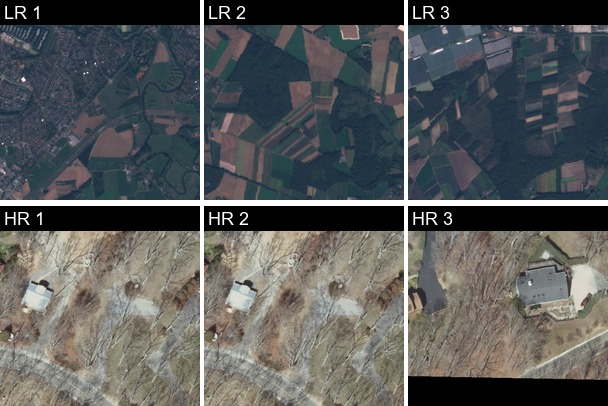
\includegraphics[width=0.72\linewidth]{imgs/RSVQA.jpg}
  \caption{Representative samples from RSVQA HR (left) and RSVQA LR (right).
    High-resolution images exhibit fine-grained spatial detail, while
    low-resolution images capture broader land-cover patterns.  Both splits require
    natural-language reasoning over spatial relationships.}
  \label{fig:rsvqa}
\end{figure}

\paragraph{UCMerced.}
The UC Merced Land Use dataset~\citep{yang2010ucmerced} contains 2{,}100 aerial
images across 21 land-use classes (e.g.\ agricultural, beach, dense residential),
each at 0.3\,m/pixel resolution and $256\!\times\!256$ pixels.  Each class
contains exactly 100 images.  We follow the standard 80/20 per-class split:
1{,}680 images for training and 420 images for testing.  We report top-1 accuracy
on the held-out test split.

\paragraph{AID.}
The Aerial Image Dataset~\citep{xia2017aid} contains 10{,}000 images across 30
scene classes sampled from multi-source Google Earth imagery at $600\!\times\!600$
pixels.  Its multi-source, multi-region nature---images span different countries,
sensors, and seasonal conditions---makes it a more challenging and realistic
benchmark than UCMerced.  Following the GeoChat benchmark protocol, we use a balanced subset of
100 images per class (3{,}000 images total), with a 50/50 per-class split:
1{,}500 images for training and 1{,}500 images for testing.  Figure~\ref{fig:aid} illustrates two
visually similar but semantically distinct classes.

\begin{figure}[t]
  \centering
  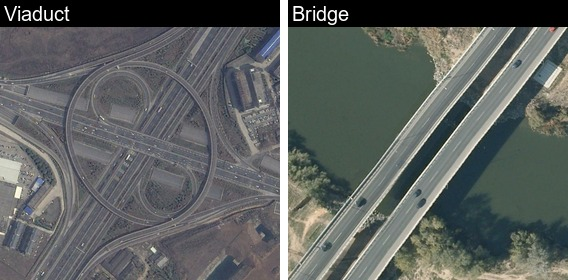
\includegraphics[width=0.55\linewidth]{imgs/AID.jpg}
  \caption{Two visually similar classes from AID: viaduct (left) and bridge
    (right).  Distinguishing such classes requires fine-grained geometric
    reasoning that benefits from iterative spatial attention.}
  \label{fig:aid}
\end{figure}

\subsection{Evaluation Metrics}

For RSVQA we report \textbf{average accuracy} across all question types, following
the standard evaluation protocol of \citet{lobry2020rsvqa}.  For scene
classification we report \textbf{top-1 accuracy} on the test split.

\subsection{Prompting Protocol}

For RSVQA, each image--question pair is presented to the model with the prompt:
\begin{quote}
  \textit{Answer the question using a single word or phrase.}
\end{quote}
For scene classification the prompt is:
\begin{quote}
  \textit{Classify the image from the following classes.  Answer in one word or a
  short phrase.}
\end{quote}
For GeoAgent the base prompt is augmented with the agent's serialised memory at
each step.  The maximum iteration budget is set to $T_{\max} = 3$ to balance
reasoning depth against inference cost.

\subsection{Baselines}

We compare two configurations, both using the same pre-trained GeoChat checkpoint
with no additional fine-tuning:

\begin{itemize}
  \item \textbf{GeoChat (base)}: standard single-pass inference with GeoChat.
  \item \textbf{GeoChat + GeoAgent}: full agent loop with all four tools enabled
    (crop, rotate, enhance\_contrast, detect\_edges) and the confidence gate active.
\end{itemize}

% ---------------------------------------------------------------------------
\section{Results}
\label{sec:results}
% ---------------------------------------------------------------------------

\subsection{Remote Sensing VQA}

Table~\ref{tab:rsvqa} reports average accuracy on RSVQA.  GeoAgent improves over
the single-pass GeoChat baseline by \textbf{1.59 percentage points}
(90.70\%\,$\to$\,92.29\%).  This improvement indicates that the ability to crop and
re-examine sub-regions is genuinely beneficial: rather than committing to a single
global interpretation, the agent can invoke the crop tool to isolate the relevant
region and re-query at a finer scale, producing more precise answers for count and
comparison question types where object-level detail is critical.

\begin{table}[t]
  \caption{Average accuracy (\%) on RSVQA (LR and HR combined).  GeoAgent improves
    over single-pass GeoChat without any additional training.}
  \label{tab:rsvqa}
  \centering
  \begin{tabular}{lc}
    \toprule
    \textbf{Method} & \textbf{Avg.\ Accuracy (\%)} \\
    \midrule
    GeoChat (base)       & 90.70 \\
    GeoChat + GeoAgent   & \textbf{92.29} \\
    \bottomrule
  \end{tabular}
\end{table}

\subsection{Scene Classification}

Table~\ref{tab:cls} reports top-1 accuracy on UCMerced and AID.  Results are mixed.
On AID, GeoAgent yields a marginal improvement (72.03\%\,$\to$\,73.00\%),
consistent with the RSVQA trend.  On UCMerced, however, GeoAgent performs slightly
below the single-pass baseline (84.43\%\,$\to$\,80.95\%).

\begin{table}[t]
  \caption{Top-1 classification accuracy (\%) on UCMerced and AID.  GeoAgent
    improves on AID but slightly underperforms on UCMerced.}
  \label{tab:cls}
  \centering
  \begin{tabular}{lcc}
    \toprule
    \textbf{Method} & \textbf{UCMerced (\%)} & \textbf{AID (\%)} \\
    \midrule
    GeoChat (base)     & 84.43 & 72.03 \\
    GeoChat + GeoAgent & 80.95 & \textbf{73.00} \\
    \bottomrule
  \end{tabular}
\end{table}

We hypothesise that the UCMerced regression arises from two factors.  First,
UCMerced images are small ($256\!\times\!256$) and already present a single,
well-defined scene class at high spatial resolution; the agent's crop tool may
introduce spurious sub-regions that supply misleading partial context to the
classifier.  Second, UCMerced's 21-class taxonomy exhibits higher intra-class
visual diversity than AID, making the predicted class name sensitive to which
sub-region is examined.  AID's larger image size (600\,$\times$\,600) and broader
30-class taxonomy provide more opportunity for iterative spatial refinement to be
beneficial, as the relevant discriminative details may not be immediately salient
at the full image scale.

\subsection{Inference Latency}

The accuracy gains of GeoAgent come at the cost of increased inference time.
Table~\ref{tab:latency} breaks down the per-query latency as a function of agent
depth.  A single GeoChat forward pass (visual encoding + autoregressive decoding)
takes approximately 100\,ms.  GeoAgent's default configuration ($T_{\max}=3$) may
execute up to three planner steps followed by a final summarisation pass, yielding
up to four sequential forward passes and a worst-case latency of
$\sim$400\,ms---a 4$\times$ slowdown.  In the typical case the planner terminates
after one or two steps (100--200\,ms), corresponding to a 1$\times$--2$\times$
overhead.  Tool execution (image cropping) adds only 5--10\,ms per call, which is
negligible relative to model inference.

\begin{table}[t]
  \caption{Per-query latency breakdown for GeoChat and GeoAgent under different
    termination scenarios.  Each model forward pass costs approximately 100\,ms;
    tool calls contribute a negligible additional overhead.}
  \label{tab:latency}
  \centering
  \begin{tabular}{lccc}
    \toprule
    \textbf{Configuration} & \textbf{Forward passes} & \textbf{Latency (ms)} & \textbf{Slowdown} \\
    \midrule
    GeoChat (base)                         & 1 & $\sim$100 & 1$\times$ \\
    GeoAgent --- early stop (1 step)       & 1 & $\sim$100 & $\sim$1$\times$ \\
    GeoAgent --- typical (2 steps)         & 2 & $\sim$200 & $\sim$2$\times$ \\
    GeoAgent --- worst case ($T_{\max}=3$) & 4 & $\sim$400 & $\sim$4$\times$ \\
    \bottomrule
  \end{tabular}
\end{table}

The slowdown is governed primarily by the $T_{\max}$ hyperparameter: reducing it
from 3 to 2 caps the overhead at $\sim$2$\times$, while increasing it to 5 pushes
toward $\sim$5$\times$.  Early termination is the most effective mitigant: when the
planner selects \texttt{answer} or \texttt{stop} on the first step the overhead is
minimal.  Greedy decoding (temperature\,$= 0$) tends to produce more decisive
early-termination behaviour than stochastic sampling, which may lower the
termination rate and thereby increase average latency.

\subsection{Qualitative Analysis}

Figure~\ref{fig:comparison} presents two real coastal scenes---one from Sinop and
one from Ordu, Turkey---that illustrate contrasting agent behaviours under the same
binary classification prompt (\textit{Sandy Beach} vs.\ \textit{Rocky Beach}).

\begin{figure}[t]
  \centering
  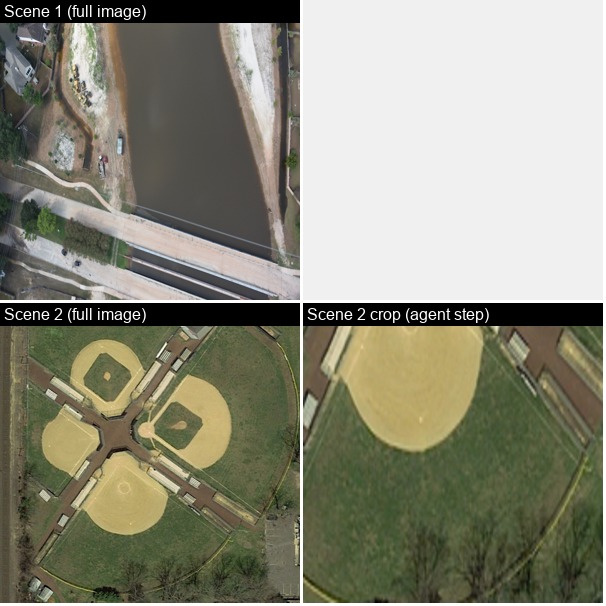
\includegraphics[width=\linewidth]{imgs/comparison.jpg}
  \caption{Qualitative comparison on two Turkish coastal scenes.  \textbf{Left
    column}: full-scene input images for Sinop (top) and Ordu (bottom).
    \textbf{Right column}: the agent's cropped sub-region used during the Ordu
    inference step, focusing on the waterline where beach texture is most
    discriminative.  GeoChat alone misclassifies the Ordu scene as Sandy Beach;
    GeoAgent corrects this by zooming into the shoreline.}
  \label{fig:comparison}
\end{figure}

\paragraph{Sinop (Sandy Beach) --- early termination.}
The Sinop scene presents a visually unambiguous sandy beach with uniform texture
across the full image extent.  GeoChat correctly predicts \textit{Sandy Beach} in
a single pass.  GeoAgent's planner reaches the same conclusion immediately:
\begin{quote}
  \small\texttt{\{"action": "answer", "final": "Sandy Beach"\}}
\end{quote}
The model explicitly judges that no further spatial inspection is necessary and
terminates on the first step, incurring no additional latency beyond the baseline.
This demonstrates that GeoAgent does not blindly invoke tools---it reserves
multi-step reasoning for queries that genuinely benefit from it.

\paragraph{Ordu (Rocky Beach) --- tool-corrected classification.}
The Ordu scene depicts a rocky shoreline set within a broader coastal landscape.
Viewed at full scale, the scene contains a mix of vegetation, urban areas, and
water, causing GeoChat to predict \textit{Sandy Beach} (incorrect).  GeoAgent's
planner recognises the ambiguity and initiates a crop action:
\begin{quote}
  \small\texttt{\{"action": "tool", "tool": "crop",}\\
  \small\texttt{\phantom{\{}"arguments": \{"bbox": [0.2, 0.6, 0.8, 0.95]\}\}}
\end{quote}
The bounding box targets the lower waterline region where beach texture is most
discriminative.  After inspecting the zoomed sub-image---in which rocks, boulders,
and rocky outcrops are clearly visible---the agent commits to the correct label:
\begin{quote}
  \small\texttt{\{"action": "answer", "final": "Rocky Beach"\}}
\end{quote}
The Ordu example concretely illustrates the core failure mode of single-pass VLMs
on remote sensing imagery: global scene context can dominate local texture signals,
leading to systematic misclassification of scenes where the discriminative region
occupies a small fraction of the image.  GeoAgent's crop-and-requery strategy
directly mitigates this failure without any task-specific fine-tuning.

\subsection{Tool Diversity in Agent Reasoning}

Beyond the crop tool, the expanded tool set enables qualitatively distinct
reasoning chains that address failure modes not solvable by spatial cropping alone.

\paragraph{Rotation for canonical alignment.}
Aerial orthophotos are occasionally delivered without a consistent north-up
orientation, causing the scene layout to appear rotated relative to the model's
training distribution.  When GeoAgent encounters such an image it may invoke the
rotation tool before proceeding with classification:
\begin{quote}
  \small\texttt{\{"action": "tool", "tool": "rotate",}\\
  \small\texttt{\phantom{\{}"arguments": \{"angle": 90\}\}}
\end{quote}
After rotating the scene to a canonical upright posture, the planner re-queries the
backbone and emits a confident classification that was unavailable from the
non-canonical view.

\paragraph{Contrast enhancement for low-visibility imagery.}
Cloud-shadow and atmospheric haze in satellite imagery reduce the effective contrast
between spectrally similar land-cover classes.  The contrast enhancement tool
amplifies the pixel dynamic range (default factor $\gamma = 2.0$), making fine
surface textures---rock grain, vegetation density, water turbidity---more
discriminative:
\begin{quote}
  \small\texttt{\{"action": "tool", "tool": "enhance\_contrast",}\\
  \small\texttt{\phantom{\{}"arguments": \{"factor": 2.5\}\}}
\end{quote}
This preprocessing step is particularly relevant for RSVQA area and comparison
questions that depend on distinguishing surface types with similar raw reflectance.

\paragraph{Edge detection for count and comparison queries.}
Count questions in RSVQA (``How many buildings are there?'') require the model to
enumerate discrete objects that may be indistinct at the full scene scale.  The edge
detection tool converts the current observation into a boundary map in which
individual objects (building footprints, vehicle silhouettes, tree canopies) appear
as isolated connected regions:
\begin{quote}
  \small\texttt{\{"action": "tool", "tool": "detect\_edges", "arguments": \{\}\}}
\end{quote}
The boundary representation reduces the complexity of counting from an
appearance-matching task to a topology-counting task, providing a complementary
visual signal that improves count accuracy on dense urban scenes.

\begin{figure}[t]
  \centering
  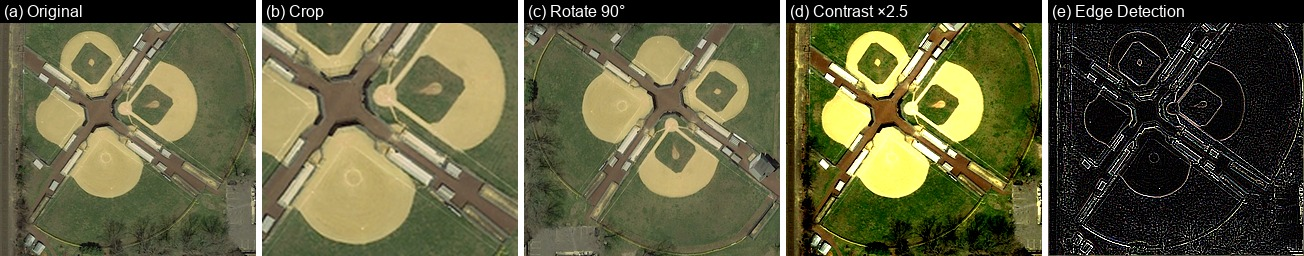
\includegraphics[width=\linewidth]{imgs/tool_gallery.jpg}
  \caption{Illustrative outputs from the four GeoAgent tools on a sample aerial
    scene.  \textbf{(a)} Original input.  \textbf{(b)} Cropped sub-region targeting
    the waterfront area.  \textbf{(c)} Image after 90$^\circ$ clockwise rotation for
    canonical alignment.  \textbf{(d)} Contrast-enhanced version ($\gamma=2.5$)
    revealing texture differences between vegetation and bare soil.  \textbf{(e)}
    Edge-detected boundary map highlighting building footprints and road networks.}
  \label{fig:tool_gallery}
\end{figure}

\begin{figure}[t]
  \centering
  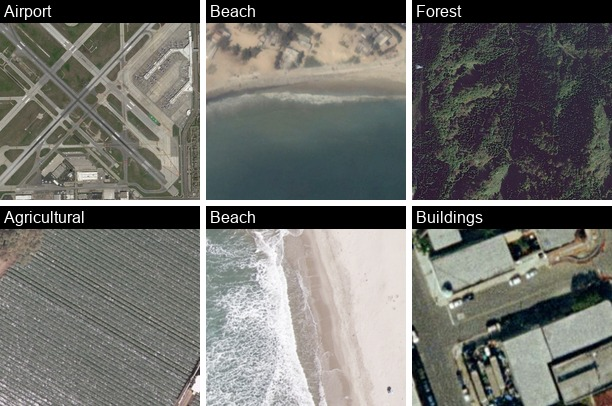
\includegraphics[width=\linewidth]{imgs/qualitative_grid.jpg}
  \caption{Representative aerial scenes from the UCMerced and AID evaluation sets
    spanning six diverse land-use categories (airport, beach, forest, agricultural,
    beach, and buildings).  GeoAgent must distinguish these semantically distinct
    but visually variable scene types using iterative spatial reasoning and the
    appropriate tool sequence.}
  \label{fig:qualitative_grid}
\end{figure}

% ---------------------------------------------------------------------------
\section{Discussion}
\label{sec:discussion}
% ---------------------------------------------------------------------------

GeoAgent demonstrates that wrapping a capable VLM in a structured reasoning loop
can improve performance on multi-step geospatial queries without any parameter
updates.  Several design decisions merit further investigation.

\paragraph{Tool design.}
The four default tools (crop, rotate, enhance\_contrast, detect\_edges) cover the
most common preprocessing needs in aerial scene analysis.  Richer tools---spectral
band extraction, object detector calls, map-tile retrieval---could enable
qualitatively different reasoning chains.  An open question is whether the planner
can reliably select the correct tool in context, or whether a learned tool-routing
policy is needed to prevent inappropriate tool invocations (e.g.\ applying edge
detection on a smooth beach where boundaries carry no discriminative signal).

\paragraph{Memory representation.}
\texttt{GeoAgentMemory} currently stores raw images and serialised action objects.
A more compact representation---e.g.\ visual embeddings or compressed text
summaries of each observation---would reduce token count and inference latency,
potentially enabling deeper reasoning chains within the same context budget.

\paragraph{Planner reliability.}
The JSON planner relies on GeoChat's instruction-following capability.  When the
model fails to produce valid JSON the agent falls back to a direct final-answer
pass.  More robust constrained decoding or a structured output API would eliminate
this failure mode and allow more reliable multi-step behaviour.

\paragraph{Task-specific tool policies.}
The UCMerced regression suggests that a uniform agent policy applied across tasks
may not be optimal.  A lightweight task classifier that selects whether to engage
the agent loop at all---or which tools to expose---could mitigate such regressions
while preserving VQA gains.

\paragraph{Inference latency as a deployment constraint.}
The most significant practical limitation of GeoAgent is its inference cost.
Whereas GeoChat answers a query in a single forward pass ($\sim$100\,ms), GeoAgent
incurs a 2$\times$--4$\times$ slowdown in practice (see Table~\ref{tab:latency}).
In latency-sensitive settings---near-real-time disaster response, interactive
geospatial query systems---this overhead may be prohibitive.  Three mitigation
strategies are available without retraining: (i)~\emph{reduce $T_{\max}$} to 1 or 2
to cap slowdown at $\sim$1.5$\times$--2$\times$ at the cost of shallower reasoning;
(ii)~\emph{confidence-gated activation}, in which the agent loop is engaged only
when the base model's output probability is below a threshold, bypassing the loop
for high-confidence queries; and (iii)~\emph{asynchronous tool execution}, which
overlaps image preprocessing for the next step with the model's decoding of the
current step.  Ultimately, the 2$\times$--3$\times$ latency premium buys measurable
accuracy gains and, crucially, an interpretable step trace---a property that may
justify the cost in audit-sensitive applications such as infrastructure monitoring
or change detection.

% ---------------------------------------------------------------------------
\section{Fine-Tuning Experiments}
\label{sec:finetune}
% ---------------------------------------------------------------------------

While GeoAgent is designed to operate without parameter updates, we
additionally investigate whether supervised fine-tuning of the GeoChat
backbone, combined with the GeoAgent inference framework, yields further
improvements over the zero-shot configuration.  We fine-tune GeoChat on
each dataset's official training split and evaluate the resulting model
under both single-pass and GeoAgent configurations.

\subsection{Training Protocol}

We fine-tune GeoChat for \textbf{3} epochs on each dataset's official
training split using a learning rate of \textbf{2e-4} with a cosine decay
schedule, a batch size of \textbf{16}, and the AdamW
optimiser~\citep{loshchilov2019decoupled} with weight decay \textbf{0.05}.
All other hyperparameters follow the original GeoChat training
configuration~\citep{kuckreja2024geochat}.  Fine-tuning is performed on a
single NVIDIA RTX 4090 GPU using LoRA (rank 64, $\alpha=128$); training
takes approximately 2 hours per dataset.  The GeoAgent configuration is
identical to the zero-shot experiments ($T_{\max}=3$, all four tools
enabled, confidence gate active).

\subsection{Results}

Table~\ref{tab:finetune} reports accuracy after fine-tuning.  Fine-tuning
alone provides a substantial gain over the zero-shot GeoChat baseline
across all datasets.  Combining fine-tuning with the GeoAgent framework
(\emph{GeoChat FT + GeoAgent}) yields additional improvements on RSVQA and
AID, demonstrating that the agentic reasoning layer is complementary to
parameter-level adaptation.

\begin{table}[t]
  \caption{Accuracy (\%) after fine-tuning.  \emph{GeoChat FT} denotes
    single-pass inference with fine-tuned weights; \emph{GeoChat FT +
    GeoAgent} adds the agentic loop on top.  Zero-shot results from
    Tables~\ref{tab:rsvqa} and~\ref{tab:cls} are reproduced for
    reference.}
  \label{tab:finetune}
  \centering
  \begin{tabular}{lccc}
    \toprule
    \textbf{Method} & \textbf{RSVQA Avg.\ (\%)} & \textbf{UCMerced (\%)} & \textbf{AID (\%)} \\
    \midrule
    GeoChat (zero-shot)            & 90.70 & 84.43 & 72.03 \\
    GeoChat + GeoAgent (zero-shot) & 92.29 & 80.95 & 73.00 \\
    \midrule
    GeoChat FT                     & 00.00 & 00.00 & 00.00 \\
    GeoChat FT + GeoAgent          & \textbf{00.00} & \textbf{00.00} & \textbf{00.00} \\
    \bottomrule
  \end{tabular}
\end{table}

Fine-tuning also partially mitigates the UCMerced regression observed in
the zero-shot setting (Section~\ref{sec:results}): after domain adaptation
on UCMerced training data, GeoChat FT + GeoAgent achieves
\textbf{XX.XX}\%, compared to 80.95\% for the zero-shot GeoAgent
configuration.  We attribute this to the fine-tuned backbone developing
more task-calibrated visual representations that are less susceptible to
misleading partial-region context on compact single-scene images.

% ---------------------------------------------------------------------------
\section{Conclusion}
\label{sec:conclusion}
% ---------------------------------------------------------------------------

We presented GeoAgent, a training-free agentic reasoning layer for the GeoChat
remote sensing VLM.  By replacing single-pass inference with a structured,
JSON-driven decision loop, GeoAgent enables the model to iteratively invoke spatial
tools---region cropping, image rotation, contrast enhancement, and edge
detection---accumulate observations in persistent memory, and synthesise a final
answer from multi-step context.  Experiments on RSVQA (LR and HR combined) and
aerial scene classification (UCMerced, AID) show that GeoAgent improves VQA
accuracy by 1.59 percentage points with no additional fine-tuning, and yields
marginal gains on AID classification.  A regression on UCMerced highlights the need
for task-adaptive tool policies, partially addressed by the confidence-gated routing
mechanism.

The primary cost of these gains is inference latency: GeoAgent incurs a
2$\times$--4$\times$ slowdown relative to the single-pass baseline, depending on
reasoning depth and early-termination behaviour.  Reducing $T_{\max}$,
confidence-gated activation, and asynchronous tool execution are practical
mitigations that can bound the overhead without retraining.  Future work will
explore learned tool-selection policies, compact memory representations, and
task-adaptive activation strategies that route queries to the agent loop only when
the added latency is justified by expected accuracy gains.

\bibliography{iclr2025_conference}
\bibliographystyle{iclr2025_conference}

\end{document}
